\documentclass{report}

% Pacotes para acentuação e formatação

\usepackage[utf8]{inputenc}
\usepackage[T1]{fontenc}
\usepackage[brazil]{babel}
\usepackage{setspace}    % Para espaçamento
\usepackage{lipsum}      % Texto de exemplo (remova se não precisar)
\usepackage{graphicx}
\usepackage{listings}
\usepackage{hyperref}





\begin{document}
	
	\begin{titlepage}
	\centering
	\vspace*{5cm} % Espaço do topo
	
	{\Huge\bfseries Arquitetura de Computadores I (LAB)\par} % Título
	
	\vspace{0.5cm}
	{\Large 2025/2\par} % Ano
	
	\vfill
	{\large Nicolas Ramos Carreira\par} % Nome
	
	\vspace*{2cm}
	\end{titlepage}
	
	\tableofcontents
	\newpage
	
	\chapter{Intuito}
	O intuito deste documento é explicar sobre o que será feito nas aulas de laboratório da disciplina de Arquitetura de Computadores I. Neste documento provavelmente estarão explicações de componentes elétricos e alguns conceitos físicos, então se prepare!
	\chapter{Fundamentos Fisicos da Computação}
	\section{Carga elétrica}
	\begin{itemize}
		\item A carga elétrica faz com que a matéria experimente uma força de atração ou repulsão
		\item A medida da carga elétrica é Coulombs (C)
		\item Para fazer uma analogia, podemos dizer que a a carga elétrica seria a água
	\end{itemize}
	\section{Corrente elétrica}
	\begin{itemize}
		\item A corrente elétrica é o movimento da carga elétrica (ou seja, representa uma taxa que mede a intensidade do fluxo elétrico)
		\item A medida da corrente elétrica é feita em Amperes (A)
		\item Em equações, costuma-se utilizar: $1A = 1 C/s$ (1 Amper = 1 Coulumb/segundo)
		\item Para fazer uma analogia, podemos dizer que a corrente elétrica seria: FLUXO DA ÁGUA EM UM PONTO/segundo
	\end{itemize}
	\section{Tensão(voltagem)}
	\begin{itemize}
		\item A tensão influencia a taxa com a qual uma carga flui através de um circuito. É a diferença de potencial elétrico entre dois pontos. Só iremos ter corrente elétrica se houver diferença de potencial.
		\item A tensão é medida em Volts (V)
		\item Para fazer uma analogia, Imagine uma fonte de energia (uma BOMBA D’ÁGUA).Essa bomba aumenta a PRESSÃO DA ÁGUA e aumenta a
		velocidade do fluxo. Essa pressão é a TENSÃO
	\end{itemize}
	\section{Resistência}
	\begin{itemize}
		\item É uma medida da dificuldade da corrente de fluir por um condutor
		\item É medida em Ohms (Ω)
		\item Uma analogia possível seria comparar com o diâmetro do cano
	\end{itemize}
	\section{Analogia(para um entendimento claro)}
	\begin{figure}[ht]
		\centering
		% ajusta a largura da imagem para ser quadrada (ex: 5cm x 5cm)
		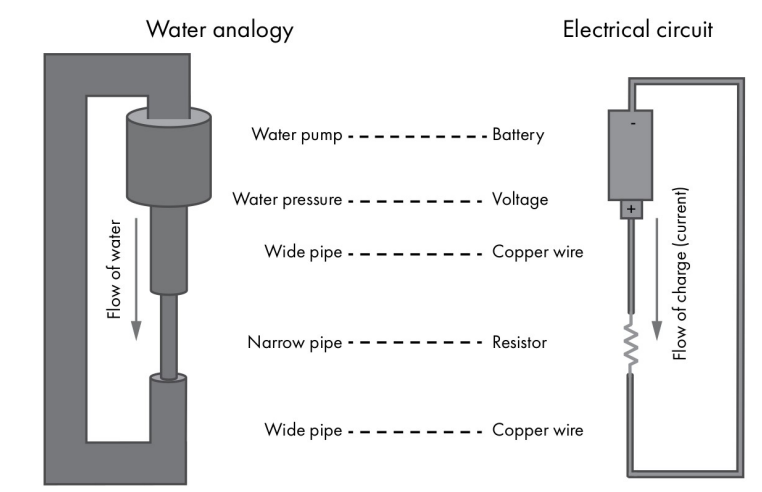
\includegraphics[width=7cm,height=5cm,keepaspectratio=false]{imagens/analogia.png}
		\caption{Water pump = Bomba d'água; Narrow pipe = tubo estreito}
	\end{figure}
	\section{Lei de Ohm}
	\begin{itemize}
		\item A lei de Ohm vai nos dizer que a corrente que flui entre dois pontos é igual à voltagem dividida pela resistência: I = V/R
		\item Seguindo com a analogia, se você aumentar a pressão da água (V), a quantidade de água que flui (I) também aumenta, desde que o entupimento (R) continue o mesmo. Por outro lado, Se o entupimento (R) for maior, a quantidade de água que flui (I) diminui, mesmo que a pressão (V) continue a mesma.
		\item CUIDADO AC X DC: A DC representa a corrente continua, que é quando A corrente flui em apenas uma direção. A maioria das pilhas e baterias usa corrente contínua (guarde esta informação). Por outro lado, temos a AC que representa a corrente alternada, onde os polos se invertem várias vezes para que a corrente continue circulando. A energia que chega nas tomadas das nossas casas é AC. É importante ter cuidado com isso pois no laboratório, durante as atividades, utilizaremos componentes que utilizam a CORRENTE CONTINUA, então não inverta o polo do capacitor na hora de encaixá-lo, pois como vimos, na corrente continua os polos não se invertem.
	\end{itemize}
	\section{Circuitos elétricos (conceitos básicos)}
	\begin{itemize}
		\item É um conjunto de vários componentes (veremos sobre esses componentes mais afrente) conectados de forma a permitir que a corrente possa fluir em um loop, a partir da fonte de energia, passando pelos elementos do circuito, e de volta à fonte de energia
		\item  Um circuito começa e termina no mesmo lugar.
		\item Em circuitos DC, o terra (GND) é considerado 0V e serve como um ponto de referência. Pode ser a terra propriamente dita, ou o polo negativo de uma bateria, por exemplo.
	\end{itemize}
	\section{Lei de Kirchhoff}
	\begin{itemize}
		\item A soma das voltagens em um circuito é 0
		\item Isso significa que se uma bateria fornece 9V para um circuito, os vários componentes do circuito devem “consumir” esses 9V. No caso da imagem abaixo, os resistores fazem esse papel
		
	\end{itemize}
	
	\begin{figure}[ht]
		\centering
		% ajusta a largura da imagem para ser quadrada (ex: 5cm x 5cm)
		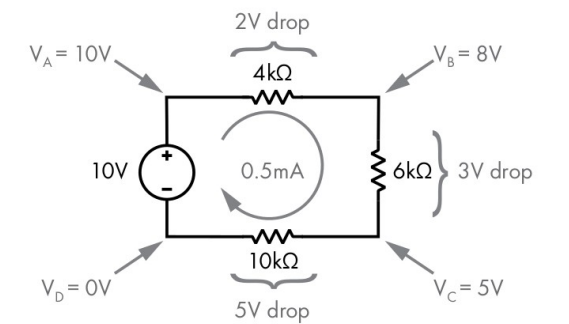
\includegraphics[width=8cm,height=5cm,keepaspectratio=false]{imagens/kirchhoff.png}

	\end{figure}
	
	Acima, os resistores irão consumir a voltagem durante o circuito, até que seja 0V. Mas afinal, como 4kΩ vira 2V, por exemplo? Para isso, usamos a fórmula V = I X R (proveniente da fórmula I = V/R). Assim teremos que:
	\begin{itemize}
		\item Corrente (I): O circuito tem uma corrente de 0.5 mA (0.0005 Amperes). corrente é a mesma em todos os resistores nesse tipo de circuito.
		\item Resistência (R): A resistência do resistor em questão é de 4k Ohms (4.000 Ohms).
	\end{itemize}
	
	Com isso, bastará fazer: V = (0.0005 A)×(4000 Ohms), que será igual a 2V. Assim, faremos isso com todos os resistores, resultando em: 2V (o primeiro que fizemos), 3V e 5V. Ao somar a voltagem de todos eles, teremos 10V. Ou seja, os resistores irão consumir a voltagem por completo, atendendo a Lei de Kirchhoff.
	
	Um detalhe é que se tivermos um circuito onde queremos descobrir qual resistor temos que colocar para que ele consuma nossa voltagem, nós usamos a fórmula R = V/I, onde vamos substituir em V quantos volts queremos que esse resistor "gaste". Em I, teremos a corrente que vai passar por esse resistor. Em circuitos simples em série, a corrente é a mesma em todos os componentes. 
	
	\chapter{Cicuito real}
	\section{O que é Arduíno?}
	Arduino é uma plataforma para auxiliar com projetos de eletronica e programação. A ideia é que você tivesse uma coisa barata, funcional (que desse para instalar coisas de verdade) e que fosse fácil de aprender. Essa plataforma é quase todo baseado em uma plaquinha. Veja a foto abaixo:
	
	\begin{figure}[ht]
		\centering
		% ajusta a largura da imagem para ser quadrada (ex: 5cm x 5cm)
		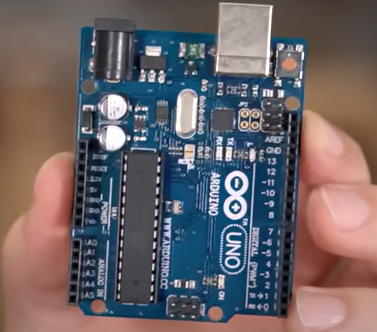
\includegraphics[width=8cm,height=5cm,keepaspectratio=false]{imagens/arduino.png}
		
		\caption{Arduino UNO R3}
		
	\end{figure}
	
	Essa plaquinha tem microcontroladores (a parte preta larga da placa que fica quase no meio) que funciona mais ou menos como um computadorzinho bem pequeno que é capaz de processar e armazenar coisas e também tem uma linguagem de programação, onde você consegue escrever coisas, criar sisteminhas que você coloca dentro e faz com que a placa te obedeça.
	
	E por que o arduino deu tão certo? Pois foi criado com a ideia de hardware livre. Qualquer um pode olhar como funciona seu circuito, comprar os componentes, montar seu próprio arduino e se quiser até vender seu próprio arduino. Isso faz com que o arduino seja barato, sendo assim usado amplamente em projetos, o que contribui para a disponibilização de vários materiais de arduino e com que várias pessoas possam ter contato com ele.
	
	Uma observação é que se pode utilizar o arduíno pela internet a partir do site TinkerCad. Se você comprar a placa, você precisa conectar ela via USB ao computador e baixar o softwere Arduino IDE, onde você bota o código que você vai fazer para enviar para a placa.
	
	Se você quiser ligar a placa sem o computador (isso acontece depois que você ja colocou o programa que voc~e fez nela), você conecta um adptador de bateria de 9V na placa por meio da entrada redonda e conecta o adaptador a bateria, aí você consegue ligar ela assim. Veja as duas entradas abaixo:
	
	\begin{figure}[ht]
		\centering
		% ajusta a largura da imagem para ser quadrada (ex: 5cm x 5cm)
		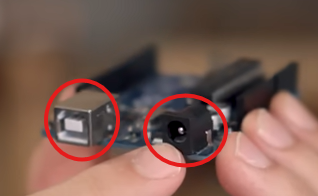
\includegraphics[width=8cm,height=5cm,keepaspectratio=false]{imagens/entradas.png}
		
		\caption{Entrada USB e entrada redonda (da esquerda para a direita)}
		
	\end{figure}
	
	O arduíno ainda possui as portas de comunicação (circulado em vermelho na imagem abaixo), que serve para espetar os fios, componentes e até outras placas (é como se fosse aquela parte lateral do computador onde tem entradas usb e de rede, por exemplo). Veja:
	
	\begin{figure}[ht]
		\centering
		% ajusta a largura da imagem para ser quadrada (ex: 5cm x 5cm)
		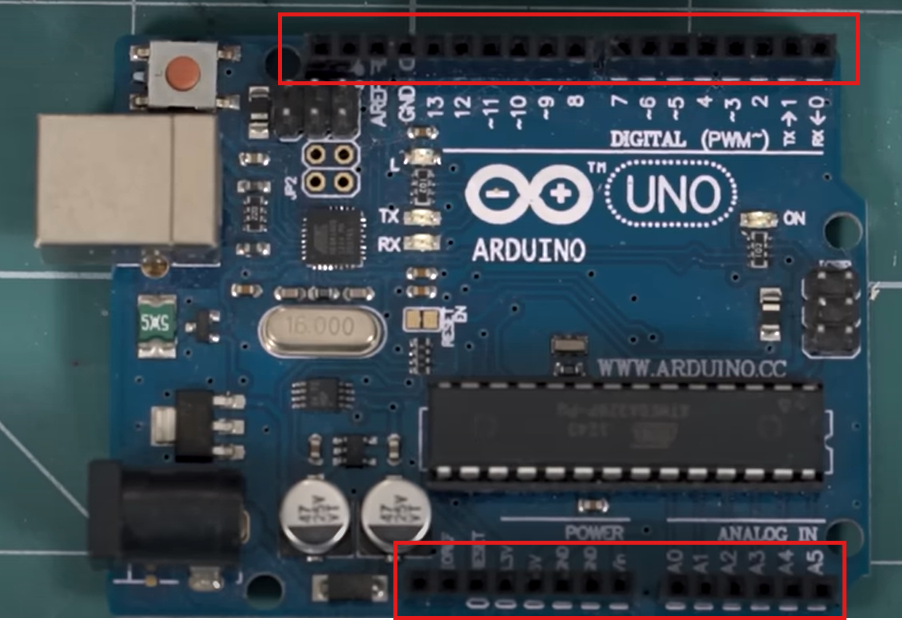
\includegraphics[width=8cm,height=5cm,keepaspectratio=false]{imagens/portas.png}
		
	\end{figure}
	
	
	Essas conexões que podemos fazer ao espetar os componentes é chamada de PINOS, sendo que podemos ter pinos de entrada e de saída. Mas como funciona isso? Suponha que você queira instalar um sensor de presença no arduíno que quando alguém chega perto, você acende um LED. O sensor irá fornecer informações para o arduino, então você coloca ele na entrada. Os pinos de saída, você usará para acender o led, pois está saindo informações do arduíno (você que define os pinos de entrada e saída no código).
	
	Alguns desses pinos tem a sigla GND, o que significa que é o TERRA.
	
	Os pinos que ficam na parte "DIGITAL" são binários, só aceitam 0 e 1. Os pinos que ficam em ANALOG" são mais espertas e identificam valores intermediários.
	
	Na parte de POWER (que é a que a gente vai usar bastante nas aulas de lab) nós temos algumas indicações de Volts, o que significa que o arduino pode ser usado para alimentar componentes
	
	
	
	\section{Principais componentes eletrônicos e ferramentas}
	
	Aqui, falaremos sobre os principais componentes e ferramentas que são utilizados em projetos arduínos. Os componentes eletronicos basicamente controlam os movimentos dos eletrons. É importante ressaltar que será dado apenas um panorama geral. 
	Iremos aprofundar conforme formos estudando os sisteminhas. Vamos a eles:
	
	\begin{itemize}
		\item Arduino Uno - É uma placa de desenvolvimento do microcontrolador que será o centro dos nossos projetos. É a peça central que orquestra e controla o funcionamento de todos os outros componentes.  \\ \\
		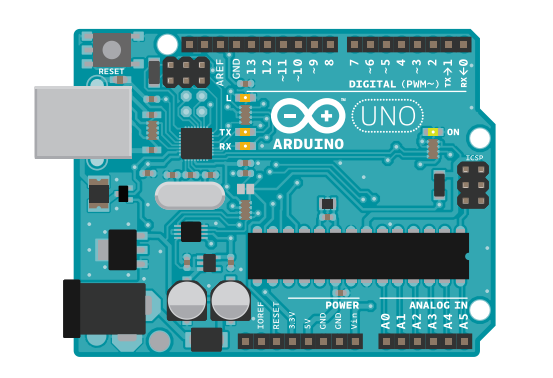
\includegraphics[width=8cm]{imagens/arduino_desenho.png}
		
		\item Snap de bateria -  É o cabo que serve para conectar uma bateria (geralmente de 9V) a um circuito, permitindo que a energia dela chegue aos componentes. (não veremos tanto por agora pois iremos conectar via usb direto no computador)\\ \\
		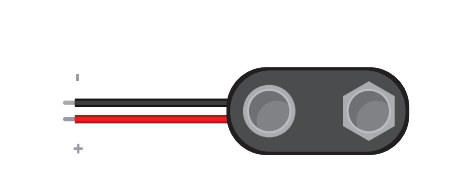
\includegraphics[width=8cm]{imagens/snap_bateria.png}
		
		\item Protoboard - É uma placa com pequenos furos que permite montar circuitos eletrônicos temporariamente, sem precisar soldar nada. Você encaixa os componentes e os fios nos furos, e pode montar, desmontar e remontar o circuito quantas vezes quiser. Os furos são interligados internamente, formando "trilhos" que levam a energia de um ponto a outro. A região do meio é divida em colunas verticais (isso com a placa deitada, como na imagem abaixo), ou seja, os 5 buraquinhos da coluna estão conectados. Na região das bordas os buraquinhos estão conectados de forma horizontal. \\ \\
		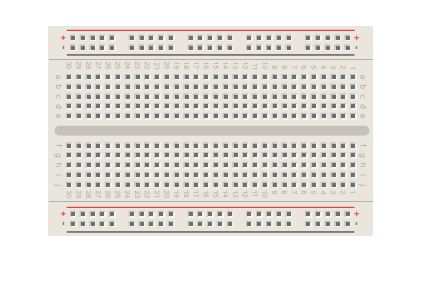
\includegraphics[width=8cm]{imagens/protoboard.png}
		
		\item Capacitores - Um capacitor armazena energia elétrica por um curto período de tempo e pode liberá-la rapidamente. Ao usar capacitores, é importante ter atenção, pois eles são polarizados (tem o polo negativo e positivo) e se conectarmos os polos no lugar errado ele pode explodir. A perna do polo negativo é destacado com uma faixa. Existem os capacitores ceramicos (o da esquerda na imagem abaixo), eletroliticos (o do meio na imagem abaixo) e de poliester (o da direita na imagem abaixo).  \\ \\
		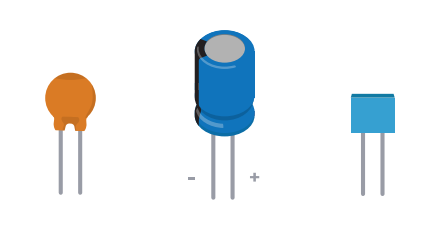
\includegraphics[width=8cm]{imagens/capacitores.png}
		
		\item Motor DC - Um pequeno motor elétrico que converte energia elétrica em movimento (rotação). Por exemplo, em um carrinho de controle remoto, é ele quem faz as rodas se moverem. \\ \\
		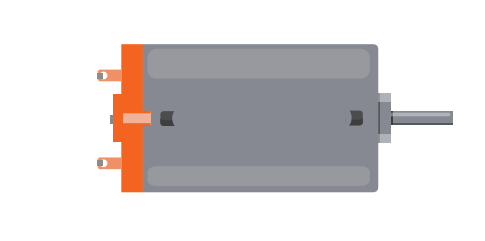
\includegraphics[width=8cm]{imagens/motor_dc.png}
		
		\item Diodo - Permite que a corrente elétrica flua em apenas uma direção. Ele bloqueia o fluxo no sentido oposto. O lado negativo do diodo é destacado por uma faixa.\\ \\
		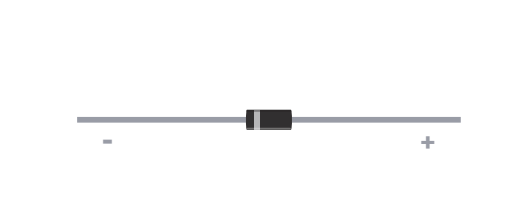
\includegraphics[width=8cm]{imagens/diodo.png}
		
		\item Fotoresistor - É um componente que muda a sua resistencia conforme a quantidade de luz que é incidida sobre ele. Quanto mais luz, menos resistencia.\\ \\
		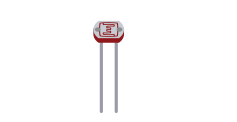
\includegraphics[width=8cm]{imagens/fotoresistor.png}
		
		\item Servo Motor - É um tipo de motor giratório que só pode rotacionar em 180 graus. É controlado pelo envio de pulsos eletricos do Arduino. Esses impulsos informam ao motor para qual posição ele deve se mover\\ \\
		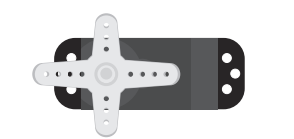
\includegraphics[width=8cm]{imagens/servo_motor.png}
		
		\item Sensor de temperatura- Altera sua saída de tensão dependendo da temperatura do componente. As pernas externas conectam-se à alimentação e
		ao aterramento. A tensão no pino central muda
		conforme esquenta ou esfria. \\ \\
		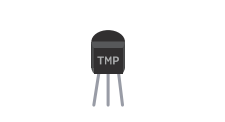
\includegraphics[width=8cm]{imagens/sensor_temperatura.png}
		
		\item Fios de ligação - São os "cabos" que você usa para conectar os componentes na protoboard. Eles criam os caminhos para a eletricidade viajar de um componente para outro na protoboard. \\ \\
		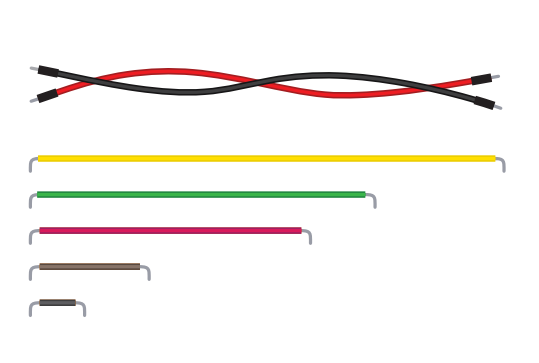
\includegraphics[width=8cm]{imagens/fios_ligacao.png}
		
		\item LEDs - É basicamente uma lâmpada. Irá emitir luz quando a corrente elétrica passa por ela. Para identificar o polo positivo pode: identificar a perna mais comprida do LED; Usar o multimetro ou identificar a parte mais gordinha do plastico do LED \\ \\
		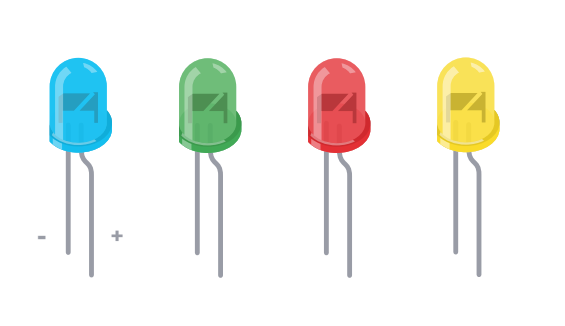
\includegraphics[width=8cm]{imagens/leds.png}
		
		\item Transistor - Funciona como um interruptor eletronico, ou seja, conseguimos ligar e desligar coisas eletronicamente. Tem 3 pernas, onde duas delas servem para a corrente fluir (o coletor e o emissor) e a terceira faz o controle (é a base).   \\ \\
		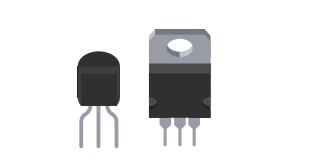
\includegraphics[width=8cm]{imagens/transistor.png}
		
		\item Botão - Um tipo de interruptor que só funciona enquanto é pressionado. Quando você o solta, ele retorna à sua posição original, interrompendo o circuito. \\
		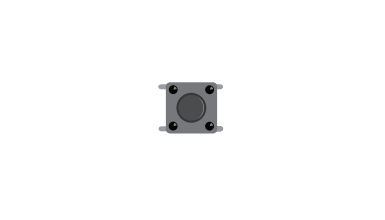
\includegraphics[width=8cm]{imagens/botao.png}
		
		\item Resistores - Ele controla e diminui o fluxo de eletricidade, como uma torneira que reduz a passagem da água. É essencial para proteger componentes como os LEDs de receberem muita corrente e queimarem. Os resistores possuem faixas coloridas que servem para indicar quantos ohms tem o resistor (qual a resitencia dele). Inclusive: \href{https://resistorcolorcode.in/?gad_source=1}{site para você ver quantos ohms tem um resistor a partir de sua sequencia de cores.} \\ \\
		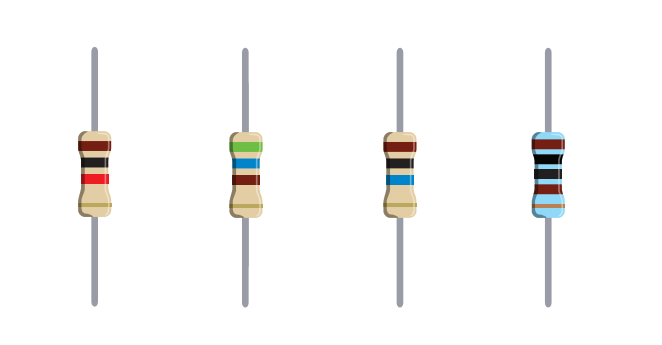
\includegraphics[width=8cm]{imagens/resistores.png}
		
		\item Potenciometros - É basicamente um resistor que você consegue variar a resistência. \\ \\
		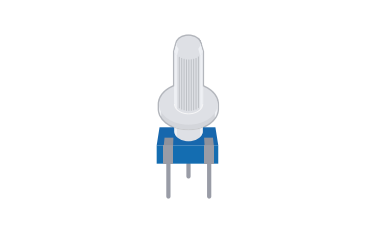
\includegraphics[width=8cm]{imagens/potenciometro.png}
		
		\item USB – É o cabo que conectaremos do computador para a nossa placa de arduíno para fornecer energia para ela e programar nela futuramente  \\ \\
		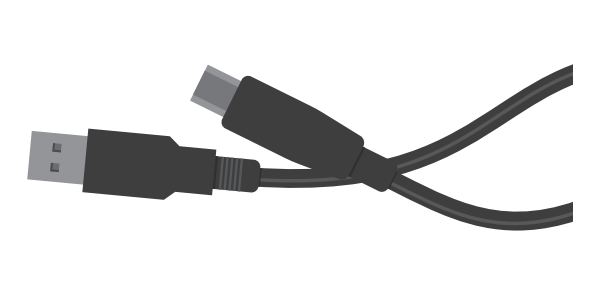
\includegraphics[width=8cm]{imagens/usb.png}
		
		\item Multimetro - É um instrumento que serve para medirmos quantos volts, qual a resistencia, se aquilo conduz energia elétrica ou não e dentre outros. Temos no multimetro dois fios, que são as pontas de prova. O preto colocamos no terra do multimetro (buraco do centro) e o vermelho, na esquerda colocamos para medir corrente (vai até 10 amperes, mais que isso ele estraga) e do lado direito volts, micro amperes e ohms, então vamos usar bem mais o lado direito. No centro do multímetro temos a chave seletora que giramos para escolher o que queremos medir. As três medidas básicas são: Volts (fica na primeira faixa cinza à direita), os Amperes (fica na faixa cinza a esquerda, debaixo da azul) e a Resistencia medida em Ohms (é a faixa onde tem o símbolo de Omega). A faixa cinza da direita serve para medir corrente alternada (para medir energia da tomada) e a faixa azul da esquerda serve para medir corrente continua (pilha, bateria e etc). O símbolo reverso  ao OFF mostra se o material está conduzindo ou não energia. Nas faixas, nós teremos os números, que significa o máximo que ele pode medir (exemplo: na faixa azul da esquerda, se colocamos no 20, significa que pode medir no maximo 20 volts)\\ \\
		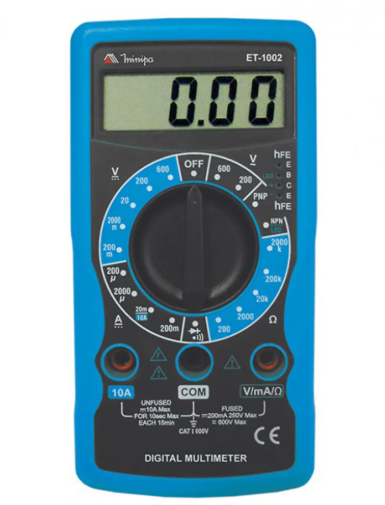
\includegraphics[width=6cm]{imagens/multimetro.png}
	\end{itemize}
	
	\section{Circuitos básicos (para entendimento)}
	\subsection{LED controlado por um botão}
	
	\chapter{Programação com o Arduíno}
	\section{Introdução}
	
	
	Quando você escreve um código em arduíno, ele sempre segue a seguinte estrutura:
	
	
	\begin{center}
		
		\begin{lstlisting}{caption=casting explicito em C, language=C, label=clanguage}
			
					
	void setup() {
		
		// aqui ficam as configuracoes que rodam 1 vez so
	}
				
	void loop() {
		// aqui fica o programa que repete para sempre
	}
	
			
		\end{lstlisting}
	\end{center}
	
	

	
	\begin{itemize}
		\item setup(): roda apenas uma vez quando a placa é ligada ou reiniciada. Usada para configurações iniciais (ex: definir pino como saída ou entrada).
		\item loop(): roda continuamente em um ciclo infinito. É aqui que o Arduino executa o programa principal.
	\end{itemize}
	
	Veja um exemplo a respeito disso:
	
		
	\begin{center}
		
		\begin{lstlisting}{caption=casting explicito em C, language=C, label=clanguage}
			
			
	void setup() {
		pinMode(13, OUTPUT); // Configura o pino 13 como saida
	}

	void loop() {
		digitalWrite(13, HIGH); // Liga LED
		delay(1000);            // Espera 1s
		digitalWrite(13, LOW);  // Desliga LED
		delay(1000);
	}

			
			
		\end{lstlisting}
	\end{center}
	

	\section{Pinos}
	
	Entender bem os pinos do Arduino é essencial porque eles são a forma de comunicação entre o microcontrolador e o mundo externo (sensores, LEDs, motores, etc.). O Arduino UNO tem 14 pinos digitais e 6 pinos analogicos. Veremos sobre eles a seguir.
	\subsection{Pinos digitais (0 a 13)}
	\begin{itemize}
		\item Podem ser configurados como entrada (INPUT) ou saída (OUTPUT) com pinMode. Exemplo: pinMode(pino, OUTPUT/INPUT).
		\item Como saída (OUTPUT) → podem enviar sinais HIGH (5V) ou LOW (0V). Exemplo: acender um LED → digitalWrite(13, HIGH);
		\item  Como entrada (INPUT) → Podem ler se há tensão (HIGH = 1) ou não (LOW = 0) em um sensor ou botão. Exemplo: ler botão → int estado = digitalRead(2);
	\end{itemize}
	
	Uma observação é que os pinos 3, 5, 6, 9, 10 e 11 têm suporte a PWM (tem um "~" ao lado do número). Isso permite simular sinais analógicos (ex: controlar brilho de LED ou velocidade de motor).
	
	\subsection{Pinos analógicos (A0 a A5)}
	\begin{itemize}
		\item Usados principalmente como entrada
		\item Leem sinais analógicos (0 a 5V) e convertem para valores digitais de 0 a 1023 através do conversor ADC (10bits). Exemplo: analogRead(A0); → retorna algo entre 0 e 1023.
		\item Muito usados com sensores que dão saída variável, como sensor de temperatura, LDR (fotoresistor), potenciômetro etc.
	
	\end{itemize}
	
	\subsection{Pinos de alimentação}
	\begin{itemize}
		\item 5V → saída de 5V para alimentar sensores e módulos.
		\item 3.3V → saída de 3.3V (para componentes que não suportam 5V).
		\item 3.3V → saída de 3.3V (para componentes que não suportam 5V).
		\item Vin → entrada de tensão quando você alimenta o Arduino com fonte externa (7 a 12V).
	\end{itemize}
	
	\section{Programando no arduíno}
	O arduíno utiliza basicamente a linguagem C, então muitas tópicos nós já sabemos, então vou passar de forma rapida em alguns deles.
	\subsection{Variaveis}
	\subsubsection{Conceito}
	Como bem sabemos, variaveis são espaços alocados na memória onde armazenamos valores. No Arduino, você usa variáveis para armazenar dados que seu programa precisa, como a leitura de um sensor, o tempo de um atraso, o estado de um LED (ligado ou desligado), ou o valor de uma porta analógica.
	
	As variaveis como também sabemos, podem assumir um tipo e cada tipo de variável tem um tamanho específico (quantos bytes ela ocupa na memória) e um intervalo de valores que pode armazenar. Dessa forma, os principais tipos do arduino e a suas utilidades são:
	
	\begin{itemize}
		\item int (inteiro): É o tipo mais comum. Armazena números inteiros, tanto positivos quanto negativos. É ideal para contadores ou para armazenar o número de um pino digital. Exemplo: int numeroDeCliques = 0;
		\item float (ponto flutuante): Usado para números que têm casas decimais. É perfeito para leituras de sensores que fornecem valores fracionários, como temperatura ou umidade. Exemplo: float temperatura = 25.5;
		\item boolean (booleano): Armazena apenas dois valores possíveis: true (verdadeiro) ou false (falso). É muito útil para armazenar o estado de algo, como "ligado" ou "desligado". Exemplo: boolean ledEstaLigado = false;
		
		
		
	\end{itemize}
	\subsubsection{Declaração e atribuição}
	
	A sintaxe para declarar e atribuir valores a variaveis em arduino segue a mesma da linguagem C:
	
	\begin{center}
		\begin{LARGE}
			tipo nomeDaVariavel = valor;
		\end{LARGE}
	\end{center}
	
	Você pode declarar a variável e atribuir um valor depois, se preferir:
	
		\begin{center}
		\begin{LARGE}
			tipo nomeDaVariavel;
			
			nomeDaVariavel = valor;
		\end{LARGE}
	\end{center}
	
	\subsubsection{Exemplo}
	
	\subsection{Operadores}
	Sabemos que os operadores são símbolos que realizam operações em valores e variáveis. Pense neles como as ferramentas básicas que você usa para fazer cálculos, comparar valores e manipular dados no seu código. No arduino os operadores são essenciais para quase tudo o que você faz em um programa, desde somar dois números até verificar se um sensor atingiu um certo valor. Falaremos então sobre cada tipo de operador
	\subsubsection{Operador aritmético}
	Esses são para operações matemáticas básicas.
	
	\begin{itemize}
		\item (Adição): Soma dois valores. Exemplo: int soma = 5 + 3; (soma será 8).
		\item (Subtração): Subtrai um valor do outro. Exemplo: int diferenca = 10 - 4; (diferença será 6).
		\item (Multiplicação): Multiplica dois valores. Exemplo: int produto = 6 * 2; (produto será 12).
		\item (Divisão): Divide um valor pelo outro. Exemplo: int quociente = 15 / 3; (quociente será 5).
		\item (Módulo): Retorna o resto de uma divisão. É útil para verificar se um número é par ou ímpar. Exemplo: int resto = 7 porct 2; (resto será 1).
		
	\end{itemize}
	
	\subsubsection{Operador de atribuição}
	Usados para atribuir um valor a uma variável.
	
	\begin{itemize}
		\item = (Atribuição simples): Atribui o valor do lado direito à variável do lado esquerdo. Exemplo: int ledPin = 13;
		\item Atribuições combinadas: Combinam uma operação com a atribuição, tornando o código mais curto.
		\begin{itemize}
			\item +=: Adição e atribuição. Exemplo: x += 5; é o mesmo que x = x + 5;
			\item -= : Subtração e atribuição. Exemplo: x -= 2; é o mesmo que x = x - 2;
			\item *=: Multiplicação e atribuição. Exemplo: x *= 3; é o mesmo que x = x * 3;
			\item /=: Divisão e atribuição. Exemplo: x /= 4; é o mesmo que x = x / 4;
		\end{itemize}
	\end{itemize}
	\subsubsection{Operador de comparação}
	Usados para comparar dois valores. O resultado de uma comparação é sempre um valor booleano: true (verdadeiro) ou false (falso).
	
	\begin{itemize}
		\item == (Igual a): Verifica se os valores são iguais. Atenção: use dois sinais de igual. Um único = é para atribuição. Exemplo: if (leitura == 100) { ... }
		\item != (Diferente de): Verifica se os valores são diferentes. Exemplo: if (estadoBotao != HIGH) { ... }
		\item > (Maior que): Exemplo: if (temperatura > 30) { ... }
		\item < (Menor que): Exemplo: if (luz < 50) { ... }
		\item >= (Maior ou igual a): Exemplo: if (contador >= 10) { ... }
		\item <= (Menor ou igual a): Exemplo: if (tempo <= 500) { ... }
		
	\end{itemize}
	\subsubsection{Operador lógico}
	Usados para combinar ou inverter resultados de expressões lógicas (as que retornam true ou false, como comparações por exemplp).
	
	\begin{itemize}
		\item \&\& (E lógico): Retorna true se ambas as condições forem verdadeiras. Exemplo: if (leitura > 100 \&\& leitura < 500) { ... }
		\item || (Ou lógico): Retorna true se pelo menos uma das condições for verdadeira. Exemplo: if (pin13 == LOW || pin12 == LOW) { ... }
		\item ! (Não lógico): Inverte o resultado. Se a condição for true, ele a torna false, e vice-versa. Exemplo: if (!sensorAtivo) { ... } (Isso é o mesmo que if (sensorAtivo == false) { ... }).
	\end{itemize}
	
	
	\subsubsection{Exemplos}
	
	\subsection{Operações condicionais}
	Como sabemos, condicionais são estruturas de controle que permitem que o seu programa tome decisões. Elas verificam se uma ou mais condições são verdadeiras ou falsas e, com base nisso, executam um bloco de código específico. No Arduino, isso é fundamental para fazer seu projeto interagir com o ambiente, como acender um LED quando um botão é pressionado, ou ligar um motor quando a temperatura sobe.
	
	\subsubsection{if}
	O if é a estrutura condicional mais básica e usada. Ela executa um bloco de código apenas se a condição for verdadeira. Sua sintaxe é:
	
	\begin{center}
		
		\begin{lstlisting}{caption=casting explicito em C, language=C, label=clanguage}	
			
	if (condicao) {
		codigo
	}
			
			
		\end{lstlisting}
	\end{center}
	
	OBS: condicao é uma expressão que retorna um valor booleano (true ou false). Geralmente, você usa os operadores de comparação (==, !=, <, >) aqui.
	
	\subsubsection{if..else}
	O if...else oferece uma alternativa: ele executa um bloco de código se a condição for verdadeira, e um bloco diferente se a condição for falsa. Sua sintaxe é:
	
	\begin{center}
		
		\begin{lstlisting}{caption=casting explicito em C, language=C, label=clanguage}	
			
	if (condicao) {
		codigo condicao verdadeira
	} 
	else {
		codigo condicao falsa
	}
			
		\end{lstlisting}
	\end{center}
	
	
	
	\subsubsection{if..else if..else}
	Essa estrutura é usada para testar múltiplas condições em sequência. A primeira condição que for verdadeira terá seu bloco de código executado, e o resto da estrutura será ignorado. Se nenhuma condição for verdadeira, o bloco else final será executado. Sua sintaxe é:
	
	\begin{center}
		
		\begin{lstlisting}{caption=casting explicito em C, language=C, label=clanguage}	
			
	if (condicao1) {
		Codigo se a condicaoo1 for verdadeira
	} 
	else if (condicao2) {
		Codigo se a condicaoo2 for verdadeira (e a 1 for falsa)
	} 
	else {
		Codigo se nenhuma das condicoes anteriores for verdadeira
	}
			
		\end{lstlisting}
	\end{center}
	
	\subsubsection{Switch..case}
	
	
	\subsection{Estruturas de repetição}
	Estruturas de repetição (ou "loops") são blocos de código que permitem executar um conjunto de instruções repetidamente, até que uma condição específica seja atendida. Elas são essenciais para automatizar tarefas que precisam ser feitas várias vezes, como ler um sensor continuamente, piscar um LED por um certo número de vezes, ou percorrer um array de dados.
	
	No Arduino, o próprio loop() principal é uma estrutura de repetição infinita que se executa indefinidamente, mas dentro dele, você pode usar outras estruturas para criar repetições mais controladas.
	
	\subsubsection{While}
	O loop while executa um bloco de código enquanto uma condição for verdadeira. A condição é verificada antes de cada execução do bloco. Se a condição começar como falsa, o código dentro do while nunca será executado. Sua sintaxe é:
	
	\begin{center}
		
		\begin{lstlisting}{caption=casting explicito em C, language=C, label=clanguage}	
	while (condicao) {
		
		codigo a ser executado repetidamente
	}
		\end{lstlisting}
	\end{center}
	
	Importante: Você deve garantir que algo dentro do loop mude a condição em algum momento, caso contrário, o loop se tornará infinito e travará o seu programa.
	
	\subsubsection{do..while}
	O loop do...while é semelhante ao while, mas com uma diferença crucial: o código dentro do loop é executado pelo menos uma vez antes que a condição seja verificada. Sua sintaxe é
	
	\begin{center}
		
		\begin{lstlisting}{caption=casting explicito em C, language=C, label=clanguage}	
	do {
		codigo a ser executado pelo menos uma vez
	} while (condicao);
		\end{lstlisting}
	\end{center}
	
	\subsubsection{for}
	O loop for é ideal quando você sabe exatamente quantas vezes a repetição precisa ocorrer. Ele é mais compacto e geralmente mais fácil de ler para repetições com um número fixo de vezes. Sua sintaxe é
	
	\begin{center}
		
		\begin{lstlisting}{caption=casting explicito em C, language=C, label=clanguage}	
	for (inicializacao; condicao; incremento) {
		codigo a ser executado repetidamente
	}
		\end{lstlisting}
	\end{center}
	Onde:
	
	\begin{itemize}
		\item inicializacao: Executada apenas uma vez, no início do loop. Geralmente é onde você declara e inicializa uma variável contadora.
		\item condicao: Testada antes de cada iteração. Se for verdadeira, o loop continua. Se for falsa, o loop é encerrado.
		\item incremento: Executado após cada iteração. Geralmente é onde você aumenta ou diminui a variável contadora.
	\end{itemize}
	
	\subsection{Monitor serial}
	\subsubsection{Conceito}
	O Monitor Serial é uma ferramenta essencial na IDE (Ambiente de Desenvolvimento Integrado) do Arduino. Pense nele como uma "janela de comunicação" que permite que o seu computador e a placa Arduino troquem dados. Ele é usado principalmente para:
	
	\begin{itemize}
		\item Depuração (Debugging): É a forma mais fácil de "ver" o que está acontecendo dentro do seu programa. Você pode imprimir o valor de variáveis, a leitura de sensores, ou mensagens de status para entender se o código está se comportando como esperado.
		\item Visualizar Dados: Se o seu projeto estiver coletando dados (como temperatura, umidade, ou leituras de sensores de distância), você pode usar o Monitor Serial para ver esses valores em tempo real no seu computador.
		\item Enviar Comandos: Você pode digitar comandos no Monitor Serial e enviá-los para o Arduino. Isso permite controlar seu projeto a partir do computador, como ligar e desligar um LED digitando "ligar" ou "desligar".
	\end{itemize}
	
	Ou seja, o Serial do Arduino é como o terminal em um programa de linha de comando (CLI) que nós fazemos em em C, por exemplo.
	
	
	\subsubsection{Como usar?}
	Para usar o Monitor Serial, você precisa de duas coisas:
	
	\begin{enumerate}
		\item Configurar a comunicação serial no seu código.
		\item Abrir a janela do Monitor Serial na IDE do Arduino.
	\end{enumerate}
	
	\begin{large}
		\textbf{Passo 1: Configurando o Código}
		\\
	\end{large}
	
	Você precisa de apenas duas linhas de código para começar a usar o Monitor Serial.
	
	\begin{itemize}
		\item Serial.begin(velocidade);
		\begin{itemize}
			\item Esta linha é colocada no bloco setup().
			\item Ela inicializa a comunicação serial.
			\item velocidade é a taxa de transmissão de dados em bits por segundo (baud rate). O valor mais comum é 9600, mas é crucial que a velocidade configurada no código seja a mesma que a escolhida no Monitor Serial.
		\end{itemize}
		\item Serial.print(); e Serial.println();
		
		\begin{itemize}
			\item Estas linhas são usadas para enviar dados do Arduino para o computador.
			\item Serial.print() imprime o dado e mantém o cursor na mesma linha.
			\item Serial.println() imprime o dado e move o cursor para a próxima linha, o que é ótimo para exibir cada informação em uma nova linha.
			\item Você pode imprimir texto, números, o valor de variáveis, etc., dentro dos parênteses.
			
		\end{itemize}
	\end{itemize}
	
	\begin{large}
		\textbf{Passo 2: Abrindo e usando a janela}
		\\
	\end{large}
	
	Depois de carregar o código na placa, siga estes passos:
	
	\begin{enumerate}
		\item Clique no ícone de lupa no canto superior direito da IDE do Arduino, ou use o atalho Ctrl + Shift + M.
		\item Uma nova janela se abrirá.
		\item No canto inferior direito, você verá um menu suspenso para a taxa de transmissão. Certifique-se de que ele esteja definido para o mesmo valor que você usou no Serial.begin() (neste caso, 9600).
		\item O Monitor Serial começará a exibir a mensagem e os valores que o seu código está enviando.
	\end{enumerate}
	
	\begin{large}
		\textbf{Dicas e considerações importantes}
		\\
	\end{large}
	\begin{itemize}
		\item Taxa de Transmissão (Baud Rate): Se a velocidade do código e a do Monitor Serial não coincidirem, você verá caracteres estranhos ou lixo eletrônico.
		\item Apenas Texto: O Monitor Serial não exibe gráficos ou imagens. Ele é feito para comunicação em texto.
		\item Alternativas: Existem ferramentas mais avançadas, como o Serial Plotter na IDE do Arduino, que transformam dados numéricos em gráficos, o que é excelente para visualizar leituras de sensores ao longo do tempo. Você pode acessá-lo no menu Ferramentas > Serial Plotter.
	\end{itemize}
	\subsubsection{Exemplo}
	\subsection{Funções}
	\subsubsection{Conceito}
	Funções são blocos de código que executam uma tarefa específica e podem ser chamados a qualquer momento no seu programa. Elas ajudam a organizar o código, torná-lo mais legível, reutilizável e fácil de dar manutenção.
	
	Pense em uma função como uma "caixa" que recebe uma ou mais informações (chamadas de parâmetros), faz um trabalho com elas e, opcionalmente, retorna um resultado. Existem dois tipos principais de funções:
	
	
	
	\begin{enumerate}
		\item Funções nativas: Aquelas que já vêm com a linguagem do Arduino, como digitalWrite(), analogRead(), delay(), etc.
		\item Funções personalizadas: Aquelas que você cria para o seu próprio projeto.
	\end{enumerate}
	\subsubsection{Por que usar}
	Usamos funções no arduino (e de modo geral) porque:
	
	\begin{itemize}
		\item Organização: Quebra um programa grande em partes menores e mais fáceis de entender.
		\item Reutilização: Se você precisa piscar um LED em diferentes partes do seu código, você pode criar uma função piscarLed() e chamá-la quantas vezes quiser, em vez de repetir as mesmas linhas de código.
		\item Legibilidade: Dar um nome descritivo a uma função (lerTemperatura()) torna o código mais claro do que ter um monte de linhas misturadas.
	\end{itemize}
	
	\subsubsection{Como criar}
	Para criar uma função, sua sintaxe é:
	
	\begin{center}
		
		\begin{lstlisting}{caption=casting explicito em C, language=C, label=clanguage}	
	tipoDeRetorno nomeDaFuncao(parametro1, parametro2, ...) {
		
		codigo que a funcao executa
		return valor; --> se retornar algo
	}
		\end{lstlisting}
	\end{center}
	
	Onde:
	
	\begin{itemize}
		\item tipoDeRetorno: Define o tipo de dado que a função vai retornar (ex: int, float, boolean). Se a função não retornar nada, use void.
		\item nomeDaFuncao: Um nome claro e descritivo para a função.
		\item parametros: Uma lista de variáveis que a função espera receber. São opcionais.
		\item return: O comando para enviar um valor de volta para onde a função foi chamada. Só é usado se o tipoDeRetorno não for void.
	\end{itemize}
	
	Um detalhe é que as funções que criamos ficam acima da parte de void setup()
	
	\subsubsection{A função map()}
	A map() re-mapeia um número de uma faixa para outra.
	
	\begin{center}
		
		\begin{lstlisting}{caption=casting explicito em C, language=C, label=clanguage}
novaVariavel = map(valor, deMin, deMax, paraMin, paraMax);
			
		\end{lstlisting}
	\end{center}
	
	Onde:
	
	\begin{itemize}
		\item valor: a variável que contém o número a ser mapeado (ex: a leitura do potenciômetro).
		\item deMin: o limite inferior da faixa original (ex: 0).
		\item deMax: o limite superior da faixa original (ex: 1023).
		\item paraMin: o limite inferior da faixa de destino (ex: 0).
		\item paraMax: o limite superior da faixa de destino (ex: 180).
	\end{itemize}
	
	
	
	\subsubsection{Exemplo}
	\subsection{Bibliotecas}
	Bibliotecas são coleções de código pré-escrito que estendem as funcionalidades do seu Arduino. Elas contêm funções e classes prontas para uso, permitindo que você adicione recursos complexos ao seu projeto sem ter que escrever todo o código do zero.
	\subsubsection{Como usar uma biblioteca}
	\begin{itemize}
		\item Incluir a Biblioteca: No inicio do seu código (sketch), você deve incluir a biblioteca com a diretiva \#include. Exemplo:
		
		
	\end{itemize}
	
	\begin{center}
		
		\begin{lstlisting}{caption=casting explicito em C, language=C, label=clanguage}
		#include <Servo.h>	

		\end{lstlisting}
	\end{center}
	
	
	\begin{itemize}
		\item Utilizar suas Funções: Após a inclusão, você pode usar as classes e funções que a biblioteca oferece.
		
		
	\end{itemize}
	
	O Arduino IDE já vem com várias bibliotecas pré-instaladas (como a Servo.h), e você pode facilmente adicionar outras através do "Gerenciador de Bibliotecas" (Ferramentas > Gerenciar Bibliotecas).
	
	
	
	
	\subsection{Alguns exemplos}
	
	\section{Uso de sensores e Saídas Analógicas}
	\subsection{LED RGB e Fotoresistores}
	\subsubsection{Uso do LED RGB}
	Um LED RGB é um único componente que contém três LEDs separados: um vermelho (R), um verde (G) e um azul (B). Veja a imagem abaixo:
	
	\begin{figure}[ht]
		\centering
		% ajusta a largura da imagem para ser quadrada (ex: 5cm x 5cm)
		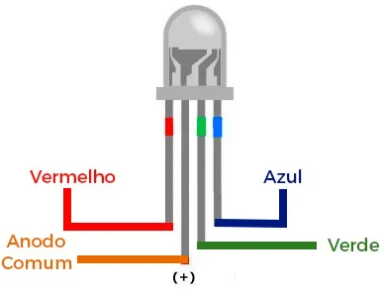
\includegraphics[width=8cm,height=5cm,keepaspectratio=false]{imagens/led_rgb.png}
		
		
	\end{figure}
	
	
	
	Ao controlar a intensidade de cada uma dessas cores primárias, você pode misturá-las para criar uma gama enorme de cores. O controle da intensidade é feito usando a técnica de PWM (Modulação por Largura de Pulso, que falaremos em breve) em cada pino de cor.
	
	\subsubsection{Uso de fotorresistores}
	Um fotoresistor, também chamado de LDR (Light-Dependent Resistor), é um tipo de sensor que muda sua resistência de acordo com a quantidade de luz que incide sobre ele. 
	
	\subsection{ Modulação por Largura de Pulso (PWM)}
	\subsubsection{PWM}
	 É uma técnica usada para simular saídas analógicas a partir de saídas digitais. O Arduino não consegue fornecer uma voltagem variável (ele só fornece 0V ou 5V), mas com o PWM ele pode ligar e desligar a saída muito rapidamente. O olho humano percebe esse "pisca-pisca" rápido como se a luminosidade fosse menor.
	 \subsubsection{Ciclo de trabalho (Duty cicle)}
	 É a porcentagem de tempo em que o sinal PWM fica em nível alto (HIGH).
	 \begin{itemize}
	 	\item Um ciclo de trabalho de 0\% significa que o sinal está sempre em LOW, e o LED fica apagado.
	 	\item Um ciclo de trabalho de 50\% significa que o sinal fica em HIGH por metade do tempo e em LOW pela outra metade, o que resulta em um brilho médio para o LED.
	 	\item Um ciclo de trabalho de 100\% significa que o sinal está sempre em HIGH, e o LED fica com o brilho máximo.
	 \end{itemize}
	\subsection{Funções analogRead() e analogWrite()}
	Já chegamos a falar um pouco dessas funções anteriormente, mas vamos revê-las porque será importante neste momento:
	
	\begin{itemize}
		\item analogRead(pino): Lê o valor de uma porta analógica (de A0 a A5) e retorna um número inteiro de 0 a 1023. Esse valor é proporcional à voltagem lida (0 = 0V, 1023 = 5V). É a função usada para ler dados de sensores como o fotoresistor
		\item analogWrite(pino, valor): Escreve um valor PWM em uma porta digital que suporte essa função (normalmente identificadas com um \~). O valor pode ser um número de 0 a 255.
		\begin{itemize}
			\item analogWrite(pino, 0) equivale a um ciclo de trabalho de 0\%, deixando o LED apagado.
			\item analogWrite(pino, 127) equivale a um ciclo de trabalho de 50\%, deixando o LED com brilho médio.
			\item analogWrite(pino, 255) equivale a um ciclo de trabalho de 100\%, deixando o LED com brilho máximo.
			
		\end{itemize}
	\end{itemize}
	
	\subsection{Sobre servos motores}
	
	Já vimos superficialmente acerca do conceito de servos motores, mas revisando: Um servo motor é um tipo especial de motor que permite controlar a posição angular do seu eixo com grande precisão. Diferente de um motor comum que gira continuamente, um servo motor pode ser instruído a mover-se para uma posição específica (um ângulo) e a manter-se firme nela.
	
	\subsubsection{Como funciona}
	
	\subsection{Capacitor de desacoplamento}
	
	Um capacitor de desacoplamento (ou decoupling capacitor) é um capacitor usado para proteger um componente ou circuito dos ruídos e flutuações da fonte de alimentação. Ele não é um tipo diferente de capacitor, mas sim uma função que um capacitor exerce.
	
	\subsubsection{Com funciona}
	
	Motores e circuitos digitais podem causar quedas repentinas e breves de tensão ao serem ligados ou ao mudarem de estado rapidamente. O capacitor de desacoplamento, posicionado o mais perto possível dos pinos de alimentação do componente que ele protege (por exemplo, um servo motor), atua como um pequeno reservatório local de energia.
	
	Quando ocorre uma queda de tensão na linha de alimentação principal, o capacitor instantaneamente fornece a energia que armazenou, "desacoplando" o componente das instabilidades da fonte. Geralmente, um capacitor eletrolítico de 100µF a 470µF é colocado entre os pinos de VCC e GND do servo motor para essa finalidade.
	
	\subsection{Potenciometro}
	
	Um potenciômetro é um resistor variável com três terminais. Ele funciona como um divisor de tensão, permitindo que você controle manualmente a voltagem de saída girando um eixo ou deslizando um cursor.
	
	

	
	
	
	
	
	
	
	 
	

	

	

\end{document}